\subsection{Diseño de muro de sótano}
Del estudio de mecánica de suelos se obtiene los siguientes parámetros geotécnicos:
\FPset\gamas{1.9}
\FPset\ko{0.431}
\FPset\kp{3.639}
\FPset\ka{0.275}
\begin{itemize}
    \item Densidad del suelo: $\gamma =\gamas\mathrm{~ton/m^3}$
    \item Coeficiente de presión en reposo: $K_{o}=\ko$
    \item Coeficiente de presión pasiva: $K_{p}=\kp$
    \item Coeficiente de presión activa: $K_{a}=\ka$
\end{itemize}
Las cotas del muro con respecto al nivel de la cara superior de cimentación de la parte mas profunda del edificio son:
\FPset\zone{3.3}
\FPset\ztwo{11.2}
\FPset\zthree{5.8}
\FPeval{\hmcon}{round(\ztwo-\zone,2)}
\begin{itemize}
    \item Cota inferior del muro: $z_{1} =\zone\mathrm{~m}$
    \item Cota superior del muro: $z_{2}=\ztwo\mathrm{~m}$
    \item Cota del segundo nivel: $z_{3}=\zthree\mathrm{~m}$
    \item Altura total del muro: $H=z_{2}-z_{1}=\hmcon\mathrm{~m}$
\end{itemize}
\FPset\wsc{2}
\FPset\wscr{0.2}
Se considero una sobrecarga de un edificio de 2 niveles en la parte posterior del muro equivalente a $w_{sc}=\wsc\mathrm{~ton/m^2}$ y una carga permanente en el primer de $w_{sc}^{\prime}=\wscr\mathrm{~ton/m^2}$.\\
Para ingresar la carga variable en ETABS es necesario definir una ecuación de la forma:
\begin{align}
    P=Ax+By+Cz+D
\end{align}
Dado que la carga solo cambia en la dirección z los coeficientes A y B resultan cero.\\
Para la presión en la parte posterior del muro se aplican las condiciones de frontera y se obtiene los coeficientes C y D:
\FPeval{\equone}{round(\ko*\wsc+\ko* \gamas * \hmcon,2)}
\FPeval{\equtwo}{round(\ko*\wsc,2)}
\FPeval{\cwall}{round((\equtwo-\equone)/(\ztwo-\zone),2)}
\FPeval{\dwall}{round(\equone-\zone*\cwall,2)}
\FPeval{\hright}{round(\zthree-\zone,2)}
\begin{align}
\shortintertext{Presión en la base del muro ($z=\zone$):} K_{o}\cdot w_{sc}+K_{o}\cdot \gamma \cdot H&=C(z_{1})+D\notag\\
\ko\cdot \wsc+\ko\cdot \gamas \cdot \hmcon&=C(\zone)+D\notag\\
\equone&=\zone\; C+D\label{eq1}\\ \shortintertext{Presión en la cota superior del muro ($z=\ztwo$):}
K_{o}\cdot w_{sc}&=C(z_{2})+D\notag\\
\ko\cdot \wsc&=C(\ztwo)+D\notag\\
\equtwo&=\ztwo\; C+D\label{eq2}
\end{align}
\noindent Combinando \ref{eq1} y \ref{eq2} se obtiene $C=\cwall\mathrm{~ton/m^3}$ y $D=\dwall\mathrm{~ton/m^2}$.\\
Se procede de manera similar para la presión que ejerce en sentido contrario el suelo de relleno debajo del segundo nivel con una altura igual a $h=z_{3}-z_{1}=\hright$.
  \begin{spacing}{2}
  \leftskip 1.27cm
  \rightskip 1.27cm
\noindent Se define el coeficiente de empuje como la relación entre la tensión efectiva horizontal y la vertical, y en el caso de que no exista deformación lateral, se denomina coeficiente de empuje al reposo, $K_{o}$. De esta forma se podría calcular el empuje sobre un muro que no se deformara lo más mínimo. Sería el caso de un muro de sótano en edificación. Pero los muros no son infinitamente rígidos, se deforman, y dependiendo de si la deformación lateral es negativa (el terreno “se descomprime”) o positiva (el terreno “se comprime”), tendríamos los denominados empujes activos $K_{a}$, o pasivos $K_{p}$, $\left ( k_{a}< k_{o} < k_{p}\right )$. Para movilizar el empuje pasivo son necesarios movimientos del muro contra el terreno muy superiores a los necesarios para llegar a una situación de empuje activo. Cuando el empuje pasivo es favorable, debido a la imprecisión en la determinación de su valor real, por seguridad suele despreciarse su efecto o bien se aplica un coeficiente reductor (por ejemplo, de 1,5). \cite{empuje}
  \end{spacing}

\begin{figure}[h!]
    \centering
    \caption{coeficientes de empujes}
    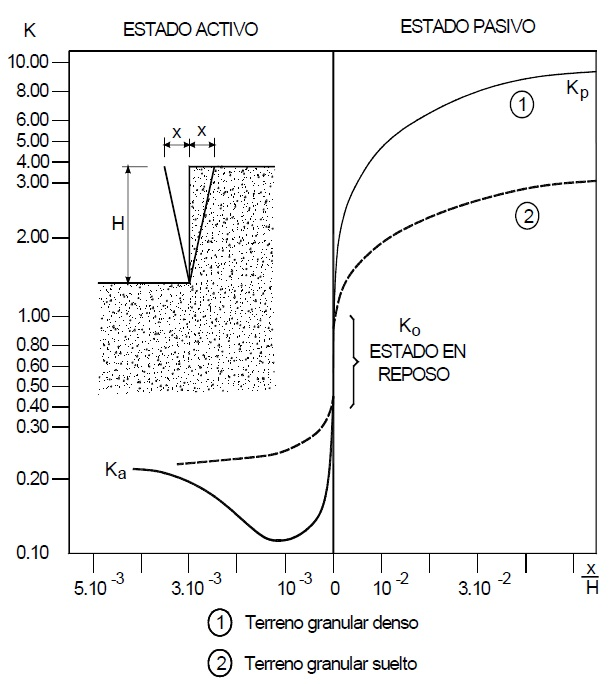
\includegraphics[scale=0.55]{IMAGENES/empuje.jpg}
    \caption*{\small Fuente: \it \cite{empuje}}
    \label{atrans}
\end{figure} 
  
\FPset\kpp{1.8}

\noindent Por lo mencionado en el anterior párrafo se hará el calculo de la presión que disminuye las solicitaciones en la pantalla del muro con un coeficiente de empuje pasivo reducido de $K_{p}^{\prime}=\kpp$
\FPeval{\equoner}{round(\kpp*\wscr+\kpp* \gamas * \hright,2)}
\FPeval{\equtwor}{round(\kpp*\wscr,2)}
\FPeval{\cwallr}{round((\equtwor-\equoner)/(\zthree-\zone),2)}
\FPeval{\dwallr}{round(\equoner-\zone*\cwallr,2)}
\begin{align}
\shortintertext{Presión en la base del muro ($z=\zone$):} K_{p}^{\prime}\cdot w_{sc}^{\prime}+K_{p}^{\prime}\cdot \gamma \cdot h&=C(z_{3})+D\notag\\
\kpp\cdot \wscr+\kpp\cdot \gamas \cdot \hright&=C(\zone)+D\notag\\
\equoner&=\zone\; C+D\label{eq3}\\ \shortintertext{Presión en el segundo nivel ($z=\zthree$):}
K_{p}^{\prime}\cdot w_{sc}^{\prime}&=C(z_{3})+D\notag\\
\kpp\cdot \wscr&=C(\zthree)+D\\
\equtwor&=\zthree\; C+D\label{eq4}
\end{align}
\noindent
Combinando \ref{eq3} y \ref{eq4} se obtiene $C=\cwallr\mathrm{~ton/m^3}$ y $D=\dwallr\mathrm{~ton/m^2}$.\\
La norma \cite{E-060} en el articulo 9.2.5 menciona que las combinaciones para el diseño de elementos sujetos a empujes de tierra sera:
\begin{align*}
    U&=1.4CM+1.7CV\\
    U&=1.4CM+1.7CV+1.7CE\\
    U&=0.9CM+1.7CE
\end{align*}
\noindent Donde:\\
CE: empuje lateral de los suelos.
\begin{figure}[h!]
    \centering
    \caption{Envolvente de momentos en la dirección horizontal de la pantalla}
    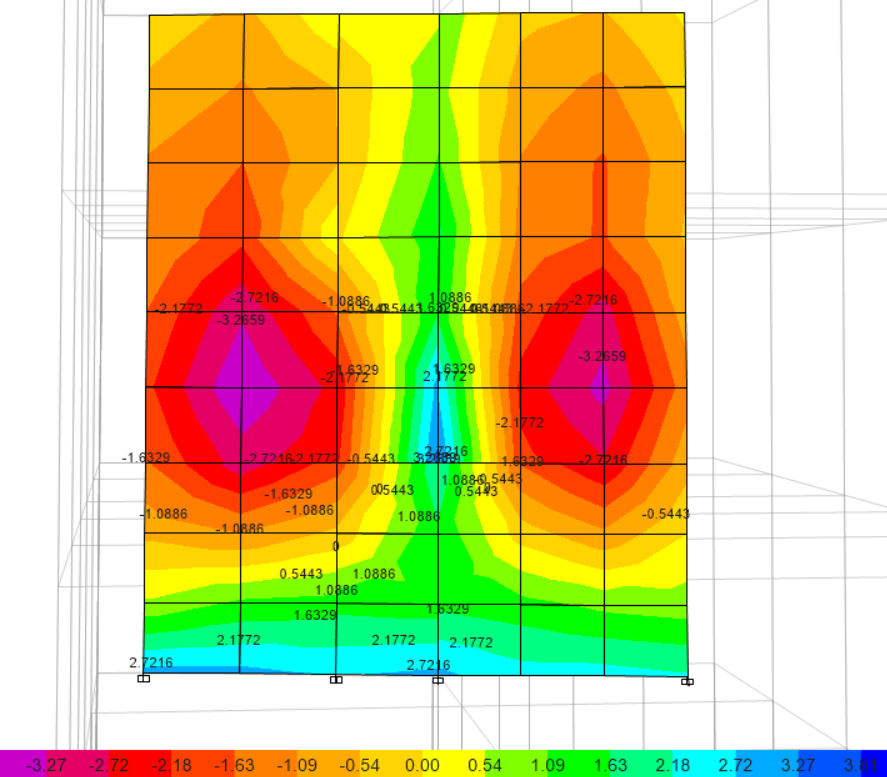
\includegraphics[scale=0.6]{IMAGENES/m11.PNG}
    %\caption*{\small Fuente: \it \cite{empuje}}
    \label{m11}
\end{figure} 

\begin{figure}[h!]
    \centering
    \caption{Envolvente de momentos en la dirección vertical de la pantalla}
    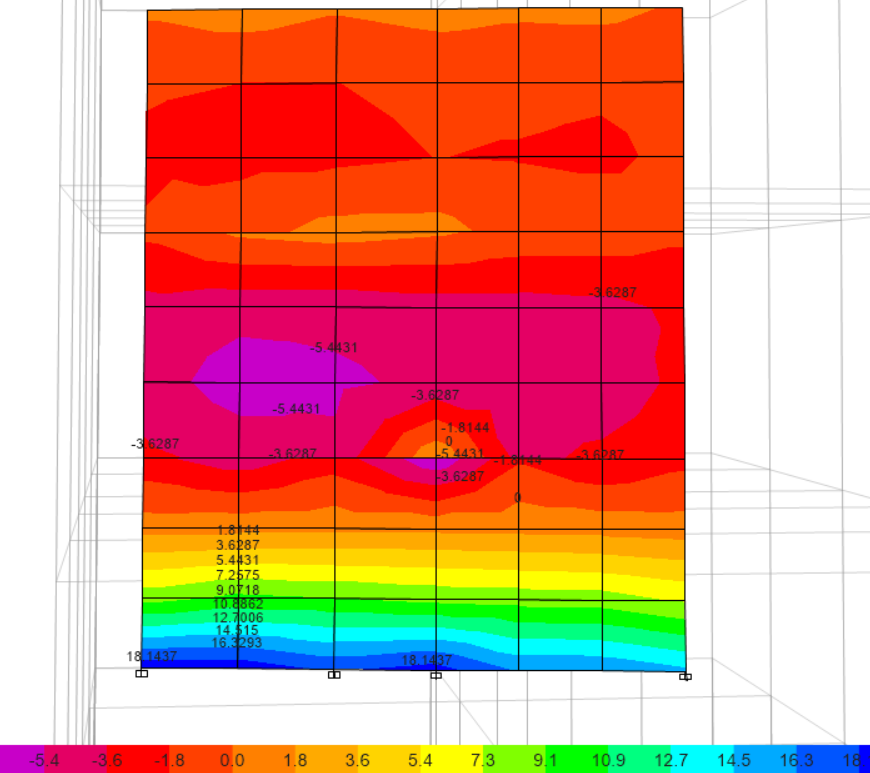
\includegraphics[scale=0.6]{IMAGENES/m22.PNG}
    %\caption*{\small Fuente: \it \cite{empuje}}
    \label{m22}
\end{figure} 
\newpage
\begin{figure}[h!]
    \centering
    \caption{Envolvente de corte de la pantalla}
    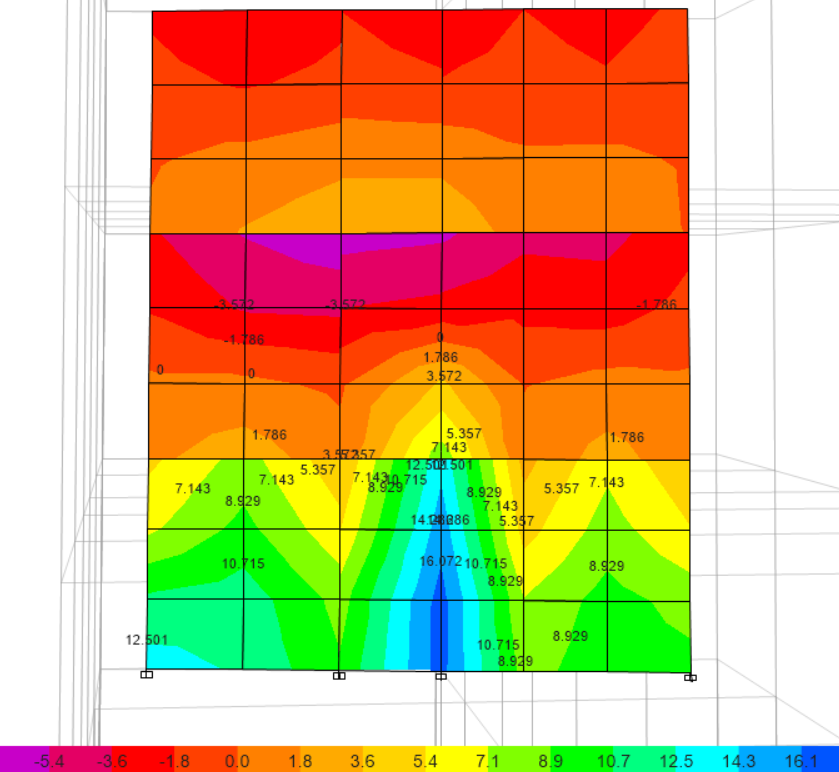
\includegraphics[scale=0.6]{IMAGENES/v23.PNG}
    %\caption*{\small Fuente: \it \cite{empuje}}
    \label{v23}
\end{figure}
\newpage
\noindent
La norma \cite{E-060} menciona en el articulo 10.5.4 que para losas estructurales donde el refuerzo se distribuye en 2 capas la cuantía mínima en la cara en tracción debe ser mayor a 0.0012.\\
Como acero horizontal se colocara doble malla de 1/2"@25cm lo que representa una cuantía de:
\FPset\shwallc{25}
\FPset\ewallc{30}
\FPset\ashwallc{1.27}
\FPset\nfhwallc{2}
\FPeval\pvwallc{round(\ashwallc/(\ewallc*\shwallc),4)}
\FPset\bwa{100}
\FPeval\ashtw{round(\ashwallc*\bwa/\shwallc,2)}
\FPeval\dwa{round(\ewallc-9,2)}
\FPeval{\mnhw}{round((0.9*\ashtw*\fy*(\dwa-\ashtw*\fy/(1.7*\fc*\bwa)))/100000,2)}
\begin{align*}
\rho_{v} =\frac{A_{sh}}{e\cdot s}=\frac{\ashwallc}{\ewallc\cdot \shwallc}=\pvwallc
\end{align*}
\noindent Para el calculo de la resistencia a la flexión de la pantalla en la dirección horizontal se considero 1m de ancho de losa y un peralte efectivo de $d=e-9\mathrm{~cm}$ dado que la norma \cite{E-060} menciona en el articulo 7.7 que el recubrimiento mínimo para concreto colocado en contacto con el suelo es mínimo 7cm.
$$
M_{nh}=\phi\cdot A_{s}\cdot f_{y}\left ( d-\frac{A_{s}\cdot f_{y}}{1.7\cdot f_{c}^{'}\cdot b} \right )$$
$$
A_{s}=\frac{A_{sh}\cdot b}{s}=\frac{\ashwallc\cdot\bwa}{\shwallc}=\ashtw\mathrm{~cm^2}$$
$$
M_{n}=0.9\cdot \ashtw \cdot \fy\left ( \dwa-\frac{\ashtw\cdot \fy}{1.7\cdot\fc \cdot \bwa} \right )=\mnhw\;\mathrm{~ton.m} 
$$
En la figura \ref{m11} se muestra que el máximo momento es de $3.72\mathrm{~ton.m}$ por lo que se cumple con $\phi M_{n}\leq M_{u}$.

Como acero vertical corrido se coloca doble malla de 5/8"@20cm:
\FPset\asvwallc{1.98}
\FPset\nfvwallc{2}
\FPset\svwallc{20}
\FPeval\asvtw{round(\asvwallc*\bwa/\svwallc,2)}
\FPeval{\mnvw}{round((0.9*\asvtw*\fy*(\dwa-\asvtw*\fy/(1.7*\fc*\bwa)))/100000,2)}
$$
A_{sv}=\frac{A_{sh}\cdot b}{s}=\frac{\nfvwallc\cdot\asvwallc\cdot\bwa}{\svwallc}=\asvtw\mathrm{~cm^2}$$
$$
M_{n}=0.9\cdot \asvtw \cdot \fy\left ( \dwa-\frac{\asvtw\cdot \fy}{1.7\cdot\fc \cdot \bwa} \right )=\mnvw\;\mathrm{~ton.m} 
$$
En la base del muro se coloca refuerzo adicional en forma de bastones con varillas de 3/4"@20cm, con lo que el momento resistente sera:
\FPset\astwallc{2.85}
\FPset\svtwallc{20}
\FPeval\asvttw{round(\asvwallc*\bwa/\svwallc+\astwallc*\bwa/\svtwallc,2)}
\FPeval{\mnvtw}{round((0.9*\asvttw*\fy*(\dwa-\asvttw*\fy/(1.7*\fc*\bwa)))/100000,2)}
$$
A_{sv}=\frac{A_{sh1}\cdot b}{s_{1}}+\frac{A_{sh2}\cdot b}{s_{2}}=\frac{\asvwallc\cdot\bwa}{\svwallc}+\frac{\astwallc\cdot\bwa}{\svtwallc}=\asvttw\mathrm{~cm^2}$$
$$
M_{n}=0.9\cdot \asvttw \cdot \fy\left ( \dwa-\frac{\asvttw\cdot \fy}{1.7\cdot\fc \cdot \bwa} \right )=\mnvtw\;\mathrm{~ton.m} 
$$
Según los resultados de la figura \ref{m22} la condición: $\phi M_{n}\leq M_{u}$ no se cumple estrictamente, pero se acepta el diseño dado las incertidumbres que conlleva el calculo de las presiones en el suelo y que se adopto valores conservadores en el calculo.\\
Así mismo se observa que el punto de corte teórico del bastón es aproximadamente 0.85m, a la cual debe sumarse el mayor valor de $12d_{b}$ y $d$ para obtener la longitud final del bastón debiéndose cumplir también sea mayor a la longitud de desarrollo $l_{d}$, con lo anteriormente mencionado se adopta un bastón de 1.10m medido desde la cara superior de la cimentación.\\
La resistencia a cortante del muro sera:
\FPeval{\vconwc}{round(0.85*0.53*\rc*\bwa*\dwa/1000,2)}
\begin{center}
$V_{c}=\phi_{c}\cdot0.53\cdot\sqrt{f_{c}^{\prime}}\cdot b\cdot d=0.85\cdot0.53\cdot\sqrt{\fc}\cdot\bwa\cdot\dwa=\vconwc\mathrm{~ton}$
\end{center}
Según los resultados de la figura \ref{v23} fuera de la zona de concentración de esfuerzos donde existe una columna la condición $\phi V_{n}\leq V_{u}$ se cumple, donde $V_{u}$ se lee a una distancia ``d'' de la cara.
\begin{figure}[h!]
    \caption{Esquema de armado en muro de contención}
    \centering
    

\tikzset{every picture/.style={line width=0.75pt}} %set default line width to 0.75pt        

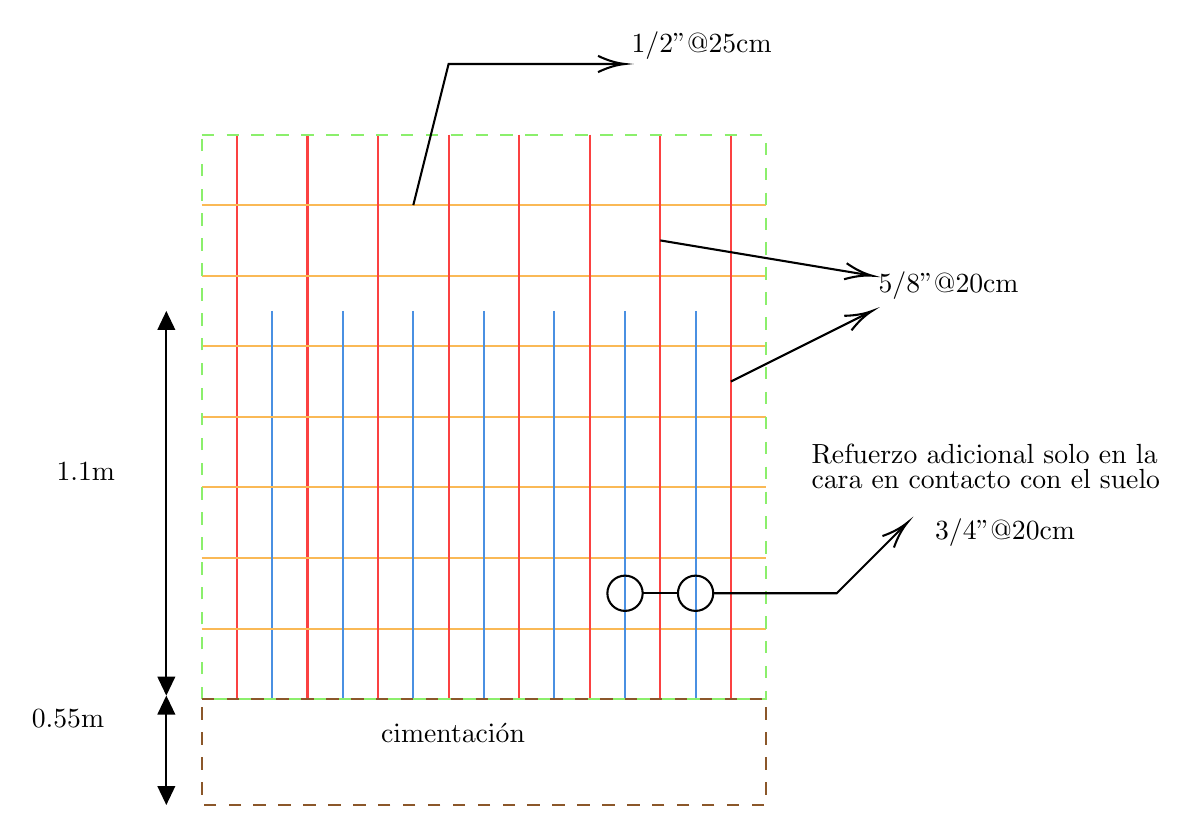
\begin{tikzpicture}[x=0.75pt,y=0.75pt,yscale=-1.7,xscale=1.7]
%uncomment if require: \path (0,294); %set diagram left start at 0, and has height of 294

%Straight Lines [id:da02765995054139414] 
\draw [color={rgb, 255:red, 251; green, 65; blue, 65 }  ,draw opacity=1 ]   (200,50) -- (200,210) ;
%Straight Lines [id:da7174171508595149] 
\draw [color={rgb, 255:red, 251; green, 65; blue, 65 }  ,draw opacity=1 ]   (220,50) -- (220,129.11) -- (220,210) ;
%Straight Lines [id:da16123548373676821] 
\draw [color={rgb, 255:red, 250; green, 185; blue, 86 }  ,draw opacity=1 ]   (190,170) -- (350,170) ;
%Straight Lines [id:da6876756264722994] 
\draw [color={rgb, 255:red, 250; green, 185; blue, 86 }  ,draw opacity=1 ]   (190,110) -- (195.44,110) -- (350,110) ;
%Straight Lines [id:da5345592683211662] 
\draw [color={rgb, 255:red, 250; green, 185; blue, 86 }  ,draw opacity=1 ]   (190,70) -- (350,70) ;
%Straight Lines [id:da4775969576589747] 
\draw [color={rgb, 255:red, 74; green, 144; blue, 226 }  ,draw opacity=1 ]   (210,100) -- (210,210) ;
%Straight Lines [id:da9167199448755778] 
\draw [color={rgb, 255:red, 250; green, 185; blue, 86 }  ,draw opacity=1 ]   (190,90) -- (350,90) ;
%Straight Lines [id:da3839448632427229] 
\draw [color={rgb, 255:red, 250; green, 185; blue, 86 }  ,draw opacity=1 ]   (190,130) -- (350,130) ;
%Straight Lines [id:da5995694819521058] 
\draw [color={rgb, 255:red, 250; green, 185; blue, 86 }  ,draw opacity=1 ]   (190,150) -- (350,150) ;
%Straight Lines [id:da5283245755076051] 
\draw [color={rgb, 255:red, 250; green, 185; blue, 86 }  ,draw opacity=1 ]   (190,190) -- (350,190) ;
%Straight Lines [id:da7631301711528842] 
\draw [color={rgb, 255:red, 251; green, 65; blue, 65 }  ,draw opacity=1 ]   (240,50) -- (240,210) ;
%Straight Lines [id:da4503876477958497] 
\draw [color={rgb, 255:red, 251; green, 65; blue, 65 }  ,draw opacity=1 ]   (260,50) -- (260,129.11) -- (260,210) ;
%Straight Lines [id:da2523584293852721] 
\draw [color={rgb, 255:red, 74; green, 144; blue, 226 }  ,draw opacity=1 ]   (250,100) -- (250,210) ;
%Straight Lines [id:da26629173415335905] 
\draw [color={rgb, 255:red, 251; green, 65; blue, 65 }  ,draw opacity=1 ]   (280,50) -- (280,210) ;
%Straight Lines [id:da47826869434014285] 
\draw [color={rgb, 255:red, 251; green, 65; blue, 65 }  ,draw opacity=1 ]   (300,50) -- (300,129.11) -- (300,210) ;
%Straight Lines [id:da6746906726566013] 
\draw [color={rgb, 255:red, 74; green, 144; blue, 226 }  ,draw opacity=1 ]   (290,100) -- (290,210) ;
%Straight Lines [id:da9467302657021419] 
\draw [color={rgb, 255:red, 251; green, 65; blue, 65 }  ,draw opacity=1 ]   (320,50) -- (320,210) ;
%Straight Lines [id:da9845424515843693] 
\draw [color={rgb, 255:red, 251; green, 65; blue, 65 }  ,draw opacity=1 ]   (340,50) -- (340,129.11) -- (340,210) ;
%Straight Lines [id:da6511672329596734] 
\draw [color={rgb, 255:red, 74; green, 144; blue, 226 }  ,draw opacity=1 ]   (330,100) -- (330,210) ;
%Straight Lines [id:da7546784093194612] 
\draw [color={rgb, 255:red, 74; green, 144; blue, 226 }  ,draw opacity=1 ]   (230,100) -- (230,210) ;
%Straight Lines [id:da9453033800840973] 
\draw [color={rgb, 255:red, 74; green, 144; blue, 226 }  ,draw opacity=1 ]   (270,100) -- (270,210) ;
%Straight Lines [id:da9828731672607554] 
\draw [color={rgb, 255:red, 74; green, 144; blue, 226 }  ,draw opacity=1 ]   (310,100) -- (310,210) ;
%Shape: Rectangle [id:dp27404908662152794] 
\draw  [color={rgb, 255:red, 139; green, 239; blue, 108 }  ,draw opacity=1 ][dash pattern={on 4.5pt off 4.5pt}] (190,50) -- (350,50) -- (350,210) -- (190,210) -- cycle ;
%Shape: Rectangle [id:dp10059166024042598] 
\draw  [color={rgb, 255:red, 139; green, 87; blue, 42 }  ,draw opacity=1 ][dash pattern={on 4.5pt off 4.5pt}] (190,210) -- (350,210) -- (350,240) -- (190,240) -- cycle ;
%Straight Lines [id:da9750542335006069] 
\draw    (180,212) -- (180,237) ;
\draw [shift={(180,240)}, rotate = 270] [fill={rgb, 255:red, 0; green, 0; blue, 0 }  ][line width=0.08]  [draw opacity=0] (5.36,-2.57) -- (0,0) -- (5.36,2.57) -- cycle    ;
\draw [shift={(180,209)}, rotate = 90] [fill={rgb, 255:red, 0; green, 0; blue, 0 }  ][line width=0.08]  [draw opacity=0] (5.36,-2.57) -- (0,0) -- (5.36,2.57) -- cycle    ;
%Straight Lines [id:da17164874403009645] 
\draw    (180,103) -- (180,206) ;
\draw [shift={(180,209)}, rotate = 270] [fill={rgb, 255:red, 0; green, 0; blue, 0 }  ][line width=0.08]  [draw opacity=0] (5.36,-2.57) -- (0,0) -- (5.36,2.57) -- cycle    ;
\draw [shift={(180,100)}, rotate = 90] [fill={rgb, 255:red, 0; green, 0; blue, 0 }  ][line width=0.08]  [draw opacity=0] (5.36,-2.57) -- (0,0) -- (5.36,2.57) -- cycle    ;
%Straight Lines [id:da36523013446236785] 
\draw    (320,80) -- (378.03,89.67) ;
\draw [shift={(380,90)}, rotate = 189.46] [color={rgb, 255:red, 0; green, 0; blue, 0 }  ][line width=0.75]    (7.65,-2.3) .. controls (4.86,-0.97) and (2.31,-0.21) .. (0,0) .. controls (2.31,0.21) and (4.86,0.98) .. (7.65,2.3)   ;
%Straight Lines [id:da881191595326331] 
\draw    (340,120) -- (378.21,100.89) ;
\draw [shift={(380,100)}, rotate = 153.43] [color={rgb, 255:red, 0; green, 0; blue, 0 }  ][line width=0.75]    (7.65,-2.3) .. controls (4.86,-0.97) and (2.31,-0.21) .. (0,0) .. controls (2.31,0.21) and (4.86,0.98) .. (7.65,2.3)   ;
%Straight Lines [id:da6470920435316516] 
\draw    (250,70) -- (260,30) -- (308,30) ;
\draw [shift={(310,30)}, rotate = 180] [color={rgb, 255:red, 0; green, 0; blue, 0 }  ][line width=0.75]    (7.65,-2.3) .. controls (4.86,-0.97) and (2.31,-0.21) .. (0,0) .. controls (2.31,0.21) and (4.86,0.98) .. (7.65,2.3)   ;
%Flowchart: Connector [id:dp48922165749553037] 
\draw   (305,180) .. controls (305,177.24) and (307.24,175) .. (310,175) .. controls (312.76,175) and (315,177.24) .. (315,180) .. controls (315,182.76) and (312.76,185) .. (310,185) .. controls (307.24,185) and (305,182.76) .. (305,180) -- cycle ;
%Flowchart: Connector [id:dp6655751446463363] 
\draw   (325,180) .. controls (325,177.24) and (327.24,175) .. (330,175) .. controls (332.76,175) and (335,177.24) .. (335,180) .. controls (335,182.76) and (332.76,185) .. (330,185) .. controls (327.24,185) and (325,182.76) .. (325,180) -- cycle ;
%Straight Lines [id:da5125267914803189] 
\draw    (315,180) -- (325,180) ;
%Straight Lines [id:da0001684757874034215] 
\draw    (335,180) -- (370,180) -- (388.59,161.41) ;
\draw [shift={(390,160)}, rotate = 135] [color={rgb, 255:red, 0; green, 0; blue, 0 }  ][line width=0.75]    (7.65,-2.3) .. controls (4.86,-0.97) and (2.31,-0.21) .. (0,0) .. controls (2.31,0.21) and (4.86,0.98) .. (7.65,2.3)   ;

% Text Node
\draw (148,142) node [anchor=north west][inner sep=0.75pt]   [align=left] {{\normalsize 1.1m}};
% Text Node
\draw (141,212) node [anchor=north west][inner sep=0.75pt]   [align=left] {{\normalsize 0.55m}};
% Text Node
\draw (240,216) node [anchor=north west][inner sep=0.75pt]   [align=left] {\normalsize cimentación};
% Text Node
\draw (311,20) node [anchor=north west][inner sep=0.75pt]   [align=left] {{\normalsize 1/2"@25cm}};
% Text Node
\draw (381,88) node [anchor=north west][inner sep=0.75pt]   [align=left] {{\normalsize 5/8"@20cm}};
% Text Node
\draw (362,140.5) node [anchor=west] [inner sep=0.75pt]   [align=left] {{\normalsize Refuerzo adicional solo en la }};
% Text Node
\draw (362,144) node [anchor=north west][inner sep=0.75pt]   [align=left] {{\normalsize cara en contacto con el suelo}};
% Text Node
\draw (397,158) node [anchor=north west][inner sep=0.75pt]   [align=left] {{\normalsize 3/4"@20cm}};


\end{tikzpicture}
    \label{fig:my_label}
\end{figure}